% Gambtt technical document (submission/doc). Text taken verbatim from the team's Claude Doc (rev 337, 2026-11-17).
% Build: tectonic Gambtt.tex
\documentclass[11pt,a4paper]{article}

\usepackage[a4paper,margin=22mm,top=20mm,bottom=22mm]{geometry}
\usepackage{fontspec}
\usepackage{microtype}
\usepackage{xcolor}
\usepackage{booktabs}
\usepackage{tabularx}
\usepackage{array}
\usepackage{enumitem}
\usepackage{titlesec}
\usepackage{needspace}
\usepackage{fancyhdr}
\usepackage{tikz}
\usetikzlibrary{positioning,arrows.meta,fit,backgrounds,calc}
\usepackage{caption}
\usepackage[hidelinks]{hyperref}

\setmainfont{texgyrepagella}[Extension=.otf,UprightFont=*-regular,BoldFont=*-bold,ItalicFont=*-italic,BoldItalicFont=*-bolditalic]
\setsansfont{texgyreheros}[Extension=.otf,UprightFont=*-regular,BoldFont=*-bold,ItalicFont=*-italic,BoldItalicFont=*-bolditalic]
\setmonofont{lmmono10-regular}[Extension=.otf,Scale=0.9]

\definecolor{ink}{HTML}{0E1A2B}
\definecolor{rule}{HTML}{C9CFD8}
\definecolor{soft}{HTML}{F2F4F7}
\definecolor{accent}{HTML}{1F5FBF}
\definecolor{home}{HTML}{1F5FBF}
\definecolor{away}{HTML}{B5462E}
\definecolor{dead}{HTML}{6B7280}

\hypersetup{colorlinks=true,linkcolor=accent,urlcolor=accent}

\titleformat{\section}{\sffamily\large\bfseries\color{ink}}{}{0pt}{}[\vspace{0.2ex}{\color{rule}\titlerule[0.6pt]}]
\titlespacing*{\section}{0pt}{2.2ex}{1.2ex}
\titleformat{\subsection}{\sffamily\normalsize\bfseries\color{ink}}{}{0pt}{}

\setlength{\parindent}{0pt}
\setlength{\emergencystretch}{3em}
\widowpenalty=10000
\clubpenalty=10000
\setlength{\parskip}{0.65ex}
\setlist{itemsep=0.25ex,topsep=0.4ex,leftmargin=1.4em}
\renewcommand{\arraystretch}{1.25}
\captionsetup{font={small,sf},labelfont=bf,skip=4pt}

\pagestyle{fancy}
\fancyhf{}
\renewcommand{\headrulewidth}{0pt}
\fancyfoot[L]{\footnotesize\sffamily\color{dead}Gambtt \textperiodcentered{} More than a Hack 2027, Phase 1}
\fancyfoot[R]{\footnotesize\sffamily\color{dead}\thepage}

\newcommand{\code}[1]{\texttt{#1}}
\newcommand{\open}[1]{\textit{#1}}

\begin{document}

% ---------------------------------------------------------------- title
{\sffamily
{\Huge\bfseries\color{ink} Gambtt: who has the ball, frame by frame\par}
\vspace{1.2ex}
{\large\color{dead} Technical document \textperiodcentered{} 17 November 2026 \textperiodcentered{} Gambtt\par}
}
\vspace{1.4ex}
{\color{ink}\rule{\linewidth}{1.2pt}}
\vspace{0.4ex}

\textbf{More than a Hack 2027, Phase 1: Ball Possession.} Repository: \href{https://github.com/TimothyBasson/mtah-2027-possession}{github.com/TimothyBasson/mtah-2027-possession}. Commit: \code{c73ac66}.

% ---------------------------------------------------------------- 1
\needspace{6\baselineskip}\section{1. Approach}

Every frame is labelled by a sticky hidden Markov model (HMM) with three states (home in possession, away in possession, dead ball), decoded with Viterbi once per half.

\begin{figure}[h]
\centering
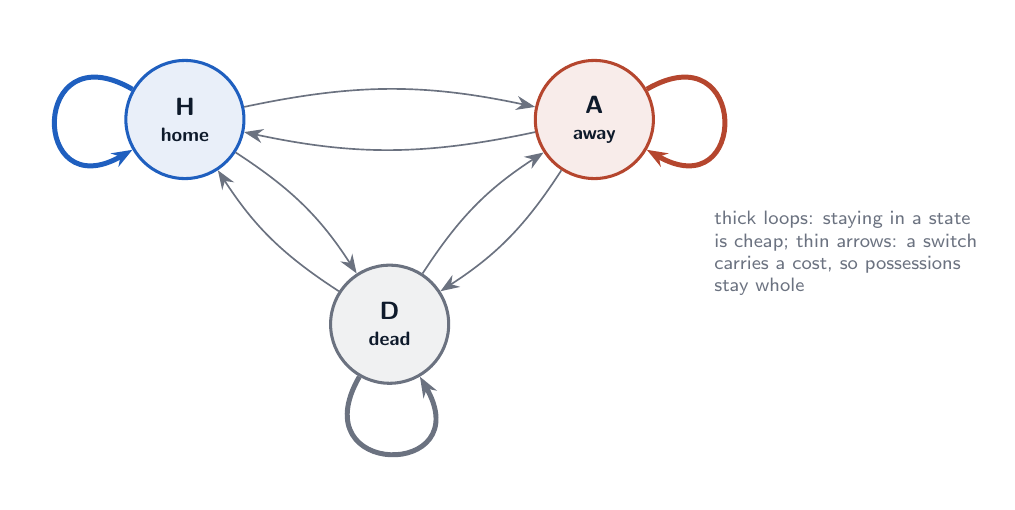
\begin{tikzpicture}[
  st/.style={circle,draw=#1,line width=1.1pt,fill=#1!10,minimum size=15mm,font=\sffamily\small\bfseries,text=ink,align=center},
  tr/.style={-{Stealth[length=2.4mm]},line width=0.6pt,draw=dead},
  self/.style={-{Stealth[length=2.6mm]},line width=1.8pt,draw=#1,looseness=5}
]
\node[st=home] (H) at (0,0) {H\\[-0.4ex]\scriptsize home};
\node[st=away] (A) at (5.2,0) {A\\[-0.4ex]\scriptsize away};
\node[st=dead] (D) at (2.6,-2.6) {D\\[-0.4ex]\scriptsize dead};
\draw[tr] (H) to[bend left=12] (A);
\draw[tr] (A) to[bend left=12] (H);
\draw[tr] (H) to[bend left=12] (D);
\draw[tr] (D) to[bend left=12] (H);
\draw[tr] (A) to[bend left=12] (D);
\draw[tr] (D) to[bend left=12] (A);
\draw[self=home] (H) to[out=150,in=210] (H);
\draw[self=away] (A) to[out=30,in=-30] (A);
\draw[self=dead] (D) to[out=240,in=300] (D);
\node[font=\sffamily\scriptsize,text=dead,align=left,anchor=west] at (6.6,-1.7) {thick loops: staying in a state\\is cheap; thin arrows: a switch\\carries a cost, so possessions\\stay whole};
\end{tikzpicture}
\caption{The three hidden states. Viterbi picks the single most likely path through them for each half.}
\end{figure}

\textbf{How we built it:}
\begin{enumerate}
  \item \textbf{Gather labelled matches.} 30 matches from three outside providers (SkillCorner 20, IDSSE 7, Metrica 3), their labels folded to the challenge's control rule (section 3).
  \item \textbf{Make them look like BAR-ATH.} The IDSSE and SkillCorner balls are knocked out to 59\% seen, so training loses the ball as often as the target match does.
  \item \textbf{Build the evidence.} Count the observation tables from those labels, train the control classifier on folded labels, and train the two players-only nets for 2,000 steps.
  \item \textbf{Keep only what helps.} Each component stays only if it improves the held-out result, with every provider judged by models that never saw it.
\end{enumerate}

Each frame's evidence is a sum of log-likelihood terms:
\begin{itemize}
  \item \textbf{Designed tracking observations}, tables counted from the outside matches' labels:
  \begin{itemize}
    \item gap and distance from the nearest home and away players to the ball
    \item where the ball is: in play, past a line, lost at a line, lost in play
    \item player speed (players walk when the ball is dead)
    \item flights: the kicker's team keeps the observation until the next touch
    \item which team is spread wider
  \end{itemize}
  \item \textbf{Control classifier}: gradient-boosted trees over 248 features, giving p(H, A, D) per frame, weight 0.2.
  \item \textbf{Two players-only nets} (\code{bt} and \code{sw25}, averaged, weight 0.3): read all 22 players, never the ball; they cover the 41\% of frames where the ball is missing.
  \item \textbf{Keeper-area observation}: a ball lost in a keeper's own box that turns up in his hands.
\end{itemize}

Two rules then adjust stoppage edges, without adding or removing possessions:
\begin{itemize}
  \item \textbf{Restart hold}: a spell after a stoppage starts at the kick of a ball that was lying still.
  \item \textbf{Keeper hold}: a short stoppage goes back to the keeper's team when he gathered the ball and play goes on.
\end{itemize}

\begin{figure}[h]
\centering
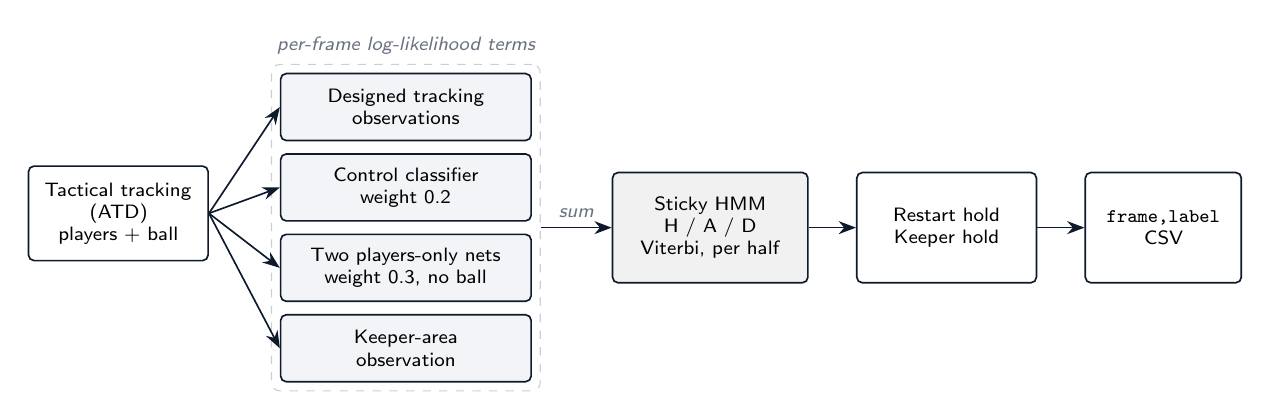
\begin{tikzpicture}[
  box/.style={draw=ink,line width=0.6pt,rounded corners=2pt,fill=white,font=\sffamily\scriptsize,align=center,inner sep=4pt},
  obs/.style={box,fill=soft,text width=29mm,minimum height=8.5mm},
  arr/.style={-{Stealth[length=2.2mm]},line width=0.6pt,draw=ink},
  lbl/.style={font=\sffamily\scriptsize\itshape,text=dead}
]
\node[box,text width=20mm,minimum height=12mm] (atd) {Tactical tracking\\(ATD)\\players + ball};
\node[obs,right=9mm of atd,yshift=13.5mm] (o1) {Designed tracking\\observations};
\node[obs,below=1.5mm of o1] (o2) {Control classifier\\weight 0.2};
\node[obs,below=1.5mm of o2] (o3) {Two players-only nets\\weight 0.3, no ball};
\node[obs,below=1.5mm of o3] (o4) {Keeper-area\\observation};
\begin{scope}[on background layer]
\node[draw=rule,dashed,rounded corners=3pt,fit=(o1)(o4),inner sep=3pt,label={[lbl]above:per-frame log-likelihood terms}] (grp) {};
\end{scope}
\node[box,right=9mm of grp,text width=22mm,minimum height=14mm,fill=ink!6] (hmm) {Sticky HMM\\H / A / D\\Viterbi, per half};
\node[box,right=6mm of hmm,text width=20mm,minimum height=14mm] (rules) {Restart hold\\Keeper hold};
\node[box,right=6mm of rules,text width=17mm,minimum height=14mm] (csv) {\code{frame,label}\\CSV};
\foreach \o in {o1,o2,o3,o4} \draw[arr] (atd.east) -- (\o.west);
\draw[arr] (grp.east) -- (hmm.west) node[midway,above,lbl]{sum};
\draw[arr] (hmm) -- (rules);
\draw[arr] (rules) -- (csv);
\end{tikzpicture}
\caption{From the tracking to the submission file.}
\end{figure}

\textbf{Why this design.} spellF1 rewards whole possessions, so an HMM with a cost for switching state avoids the fragmented possessions that per-frame classifiers produce.

We considered three alternatives first. \textbf{Fixed if-then rules per frame} (such as ``nearest player has the ball'') are simple, but a rule can't weigh weak evidence, and the ball is missing on 41\% of graded frames. \textbf{Per-frame classifiers with smoothing} read each frame well, but short smoothing windows still fragment possession. \textbf{Players-only neural nets} work without the ball, but on their own they do worse held out than when combined with the other observations.

We landed on an \textbf{HMM} because it weighs observations of different strength in one decoder, charges a cost for switching team so possessions stay whole, and takes each new observation as an extra term, kept only if it helps held out.

% ---------------------------------------------------------------- 2
\needspace{6\baselineskip}\section{2. Assets used, and how}

The labels come from the tactical-camera tracking alone; the other assets are used for checks or not at all.

\begin{center}
\small
\begin{tabularx}{\linewidth}{@{}>{\raggedright\arraybackslash}p{38mm}>{\raggedright\arraybackslash}p{26mm}>{\raggedright\arraybackslash}X@{}}
\toprule
\sffamily\bfseries Asset & \sffamily\bfseries Used? & \sffamily\bfseries How \\
\midrule
Tactical-camera automatic tracking (ATD) & yes, the only input & players and ball positions for every observation, the control classifier and the nets (the nets read the players only) \\
Smart Tagging & kickoff frames; checks & the published kickoff frames pin graded frames before each kickoff to dead ball; the tagged set pieces are printed beside decoded restarts as a diagnostic, never used to set a label \\
Broadcast tracking & no & \\
Homography & no & the ATD already gives pitch positions (normalised 0-1, scaled to a 105.3 x 68 m pitch); homography only maps them to video pixels \\
Video & no & \\
\bottomrule
\end{tabularx}
\end{center}

\textbf{Tried and dropped.} Each idea below was tested on the outside matches, held out by provider, and left out because it did not raise spellF1:
\begin{itemize}
  \item Letting the control classifier replace the gap and flight observations, rather than adding to them: worse on every provider.
  \item Making a change of team cheaper wherever a second classifier spots a change of possession: it helped against the raw labels but not the folded ones, and it hurt SkillCorner.
  \item Feeding the nets' outputs into the control classifier as 45 extra features: 0.658, well below adding the net to the decoder directly (0.674 with one net).
  \item A look-ahead observation that judges each gap where the ball is missing by where the ball reappears: it fixed some false stoppages but lowered the held-out score overall, so only its keeper part was kept (the keeper-area observation).
  \item Two clean-up rules: merging very short possessions into the team on either side, and turning short spells between two stoppages into dead ball. Both were flat or worse.
\end{itemize}

% ---------------------------------------------------------------- 3
\needspace{6\baselineskip}\section{3. Training data}

Every learned part of the model (the observation tables, the control classifier and both nets) is trained on the same 30 outside matches.

\begin{center}
\small
\begin{tabularx}{\linewidth}{@{}>{\raggedright\arraybackslash}p{24mm}>{\raggedright\arraybackslash}X>{\raggedright\arraybackslash}p{40mm}>{\raggedright\arraybackslash}p{26mm}@{}}
\toprule
\sffamily\bfseries Dataset & \sffamily\bfseries Source and licence & \sffamily\bfseries Labelled by & \sffamily\bfseries Amount \\
\midrule
SkillCorner open data & \href{https://github.com/SkillCorner/opendata}{SkillCorner/opendata}, MIT; A-League 2024-25 & the provider: phases of play and per-frame possession group & 20 matches \\
IDSSE & \href{https://huggingface.co/datasets/pysport/idsse-data}{pysport/idsse-data}, CC BY 4.0; Bassek et al., Scientific Data 12, 195 (2025) & DFL data operators: per-frame BallStatus and BallPossession & 7 matches (2 Bundesliga, 5 second-division, 2022-23) \\
Metrica sample data & \href{https://github.com/metrica-sports/sample-data}{metrica-sports/sample-data} at commit \code{e706dd5} & rebuilt by our code from the provider's event data & 3 matches \\
\bottomrule
\end{tabularx}
\end{center}

\textbf{How the labels are used.} None of the three sources applies the challenge's exact controlled-possession rule. DFL's labels flip on a first touch, so 20-30\% of their possessions are under 2s. We therefore also score against \textbf{folded} labels (external/control.py), which hand brief touches back to the team that had the ball.

To make the outside be more indicative of BAR-ATH, the IDSSE and SkillCorner balls are knocked out to 59\% seen with a fixed-seed dropout before features are computed. SoccerTrack v2 (8 matches, CC BY 4.0) was tried as a fourth training source for the nets and not kept.

% ---------------------------------------------------------------- 4
\needspace{6\baselineskip}\section{4. Possession rules implemented}

Possession changes only when the other team gains control as per the documented specification.
\begin{itemize}
  \item \textbf{Loose balls:} possession passes on control, not on the first touch. During a flight the kicker's team keeps the evidence until the next touch, so a long ball changes possession where it lands, not where it was struck. A ball with nobody near it is weak evidence for either team and leans towards a stoppage.
  \item \textbf{Challenges and duels:} the HMM's cost for changing state, and a control classifier trained on folded labels (under 2s and under 2 touches is not a change), keep possession with the team in control through a deflection or a contested touch. Very short possessions are not removed, it was measured and was flat.
  \item \textbf{Restarts and stoppages:} a frame is dead ball when the ball is seen past a line or lost at one, when the players walk, or when nobody is near it. Graded frames before each half's kickoff are dead. After a stoppage, possession starts at the kick of a placed ball (restart hold). A keeper holding a ball the tracker has lost is his team's possession, not a stoppage.
  \item \textbf{Abstentions:} the file writes \code{X} only outside the two halves' playing windows (before kickoff, half-time, after the final whistle). Every frame inside them gets \code{H}, \code{A} or \code{D}.
\end{itemize}

% ---------------------------------------------------------------- 5
\needspace{6\baselineskip}\section{5. Limitations}

The weakest part is naming the team in short possessions where the ball is missing. All numbers here are from the outside matches.
\begin{itemize}
  \item \textbf{Short possessions of the other team.} Held out, most spell errors are 2-5 s possessions of the other team. That is team-naming quality, not a timing bias a rule can move.
  \item \textbf{Broadcast-style tracking.} SkillCorner, tracked from broadcast video, scores 0.496 against 0.727 and 0.807 for the other two.
  \item \textbf{Restarts the hold cannot reach:} throw-ins (the ball moves with the thrower) and restarts with the ball unseen.
  \item \textbf{Reproducibility across CPUs.} Two runs on one machine give the same bytes; the file has not been regenerated on a second CPU, and the nets' last bits could differ between instruction sets.
\end{itemize}

\textbf{With more time:} better team naming in short ball-missing possessions; calibrating the dead-ball call to this tracker's ball dropouts; training a model to predict where the ball is on every frame, so the decoder always has a ball position even when the tracker loses it; a regeneration check on a second machine.

% ---------------------------------------------------------------- 6
\needspace{6\baselineskip}\section{6. Reproduction}

One command builds, validates and fingerprints the file. It runs on a CPU; no GPU is needed.
\begin{enumerate}
  \item \textbf{Data:} unpack the organisers' bundle into \code{data/} (data/README.md). Only the tactical tracking, its metadata and Smart Tagging are read.
  \item \textbf{Environment:} Python 3.11, then \code{pip install -r requirements.txt -r requirements-deep.txt} (numpy, pandas and torch 2.15.0, pinned; \code{uv.lock} pins every version).
  \item \textbf{Build:} \code{python submission/make\_submission.py --twice}. It runs \code{python -m hmm.decode}, runs the organisers' validator, checks that two runs give identical bytes and writes \code{submission/out/Gambtt.csv} with a manifest of its sha256, commit and library versions.
\end{enumerate}

The committed models are read, not retrained: \code{hmm/models/control\_state.npz}, \code{deep/models/bt.pt} and \code{deep/models/sw25.pt}. Retraining is documented (external/README.md) but a refit is not byte-identical, so the file is reproduced from the committed models.

The submitted \code{Gambtt.csv} was built with Python 3.11.18, numpy 2.4.6, pandas 3.1.0 and torch 2.15.0.

\noindent{\small Commit: \code{c73ac66b1bdf393e4c47cc5260f7d700e3a678f9}\\
sha256: \code{26f1cbce423f604fe358e9c013a1acabc28c48a012d66bf202f6a13e951a35f4}}

\end{document}
